\documentclass[12pt]{article}

\usepackage[english]{babel}
\usepackage{geometry}
\usepackage{titlesec}
\usepackage{graphicx}
\usepackage{placeins}
\usepackage{amsfonts}

\usepackage{amsmath}
\usepackage[style=ieee, dashed=false]{biblatex}



\geometry{a4paper, margin=1in}

\addbibresource{bib.bib} 


\begin{document}


\title{\textbf{\Huge CheapChips: A self-sustaining decentralized lottery app }}

\author{\normalsize Łukasz Tumiński (el-tumero) \\ \small tumerpl@gmail.com}
\date{}
\maketitle


% tutaj mozna napisac o tym ze loterie moga miec wiele niejasnosci a siła blockchaina
% oraz rozproszonych obliczeń oraz kryptografii pomogła nam uzyskać w pełni niezalezna
% system loterii zabezpiecznony weryfikowalna funkcja losowa

\begin{abstract}
An automated, decentralized online lottery would allow taking part in fully transparent lotteries whose result cannot be altered by any party. A game of this kind can be made using blockchain supporting smart contracts and blockchain oracles providing Verifiable Random Function (VRF).
\end{abstract}


\section{Introduction}
Online games of chance often rely on some source of randomness, which is hard to or cannot be verified at all. In a centralized environment, the consumer has to trust third parties who are responsible for selecting the winner. This is far from ideal. A non-verifiable random number generator can easily become just seemingly random due to it being controlled by a third party. This leaves a problem of possible implementation of undisclosed business strategies.

Thanks to the power of blockchain and cryptography online games of chance can be revolutionized by implementing solutions where trust is no longer needed. For this to happen, the code of a specific game must be open-sourced and its implementation must be placed on the blockchain as a smart contract\cite{smartcontract}. It would also have to use a Verifiable Random Function (VRF) to provide truly random results.

In our project we decided to create EVM-compatible smart contracts where the game (lottery) mechanics are implemented. We chose to build on EVM\cite{evm} because currently EVM-chains are the most popular and they also support Chainlink services.
Chainlink\cite{chainlink} is a Web3 services platform which helps developers to introduce smart contract functionalities, which are not natively supported on-chain. We integrated our project with Chainlink VRF\cite{vrf} for on-chain randomness and Chainlink Automation\cite{automation} for on-chain automation, which makes end-user experience much better.

% trzeba dopisac ze tutaj celujemy najpierw w male kwoty i w przyszlosci bedzie umozliwiona modyfikacja stałych takich jak max liczba graczy, max pula itd

\newpage
\section{Implementation}
\subsection{Jackpot}

Our app presents a game of chance design called \textbf{jackpot}. We define \textbf{jackpot} as a game where players increase the prize pool by placing bets. The chances of winning the entire prize pool are linearly proportional to the size of the bet.

Our jackpot runs in independent \textbf{rounds}. This is what a life-cycle of a single round looks like:

\begin{itemize}
    \item Round is created
    \item Round opens deposits (bets)
    \item After the minimum number of players criteria is met, deposit end time (timestamp) is set 
    \item When the deposit end time is reached - deposit closes
    \item Round awaits for VRF-generated result to determine round winner
    \item After the round winner is determined - round ends
\end{itemize}

The minimum number of players in a round is the amount of players required to close the deposit and thus end the round. It's a constant value.

\hfill

\textbf{Round} occurs in three states:
\begin{itemize}
    \item DEFAULT - round state before closing the deposit
    \item CLOSED - round state after closing the deposit, awaiting VRF-generated random result
    \item ENDED - round has ended and round winner is determined
\end{itemize}

\hfill

The entire logic is implemented inside CheapChipsJackpot smart contract.

\subsubsection{Deposit}

During the \textbf{DEFAULT} round state players can call the Deposit function of Jackpot contract, which transfers special tokens called \textbf{ChipStable} (the game currency) from the player's account to the Jackpot contract. After that, the contract generates an id for each player (unique number identifier). An id is genererated for every participant each round, which means a player's id might differ each round. The amount of \textbf{ChipStable} tokens a player has deposited into the round prize pool is later represented as their tickets. A ticket is an integer equal to the player's id and represents one \textbf{ChipStable} that the player has deposited. Tickets are stored together inside an array, whose length represents how many tokens are inside the rounds prize pool.  

\newpage

\textbf{EXAMPLE}:

Address 0xBA...d4e8 deposits 3 tokens into the round - they are the first player to join this round, so the contract gives address 0xBA...d4e8 id = 0, the tickets array is then set to [0,0,0]

Address 0x16...b477 deposits 2 tokens into the round - one player already participates in this round, so the contract gives address 0x16...b477 id = 1, the tickets array is then set to [0,0,0,1,1]

Address 0x16...b477 deposits 1 tokens into the round - there are already 2 participants in this round, so the contract gives address 0x16...b477 id = 2, the tickets array is then set to [0,0,0,1,1,2]

\begin{figure}[!ht]
    \centering
    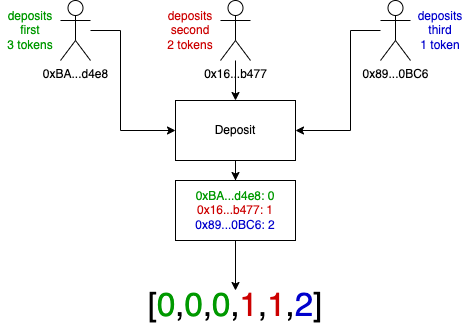
\includegraphics[scale=0.6]{images/deposit.png} 
    \caption{Deposit example visualization}
    \label{fig:b1}
\end{figure}
\FloatBarrier

% minimum-players-in-round
After meeting the requirement of minimum number of players in round, calling Deposit function will also set the timestamp after which deposit for that round will close.

In order to deposit, a player must also pay a fee in LINK token. This concept will be later discussed in [section 2.1.5].

\subsubsection{Close round}

Closing the Jackpot round will also close the deposit for the current round.

Ideally, the round should close itself after a specified period of time (when current timestamp is greater than round closing timestamp). This is not achievable natively on EVM due to lack of self-executing contracts or delayed calls. A player would have to close the round manually, and thus would be charged additional gas fees for performing the transaction. This goes against the goal of automating the round life-cycle.
A solution for this problem is to use Chainlink Automation service instead. This service can fully automate the call of the close round function.

\hfill

The close round function changes contract state to \textbf{CLOSED} and sends a request for a random number to the VRF Coordinator (Chainlink VRF).

\subsubsection{End round}
The VRFCoordinator calls the fulfilRandomWords function, where the random number (verified on-chain) is passed to the Jackpot contract. Then, Jackpot contract adds the random number to round data, sets round state to \textbf{ENDED}, and emits a RoundEnded event. Finally, the deposit is opened for a new (next) round.

The winner id of the round can be determined by using following operations:

\[ winner\;index = random\;number\mod tickets\;length \]
\[ winner\;id = tickets[winner\;index] \]

\begin{figure}[!ht]
    \centering
    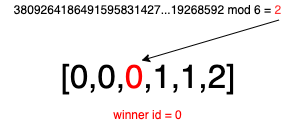
\includegraphics[scale=0.8]{images/winnerId.png} 
    \caption{Winner id}
    \label{fig:b1}
\end{figure}
\FloatBarrier

It is worth mentioning that performing the modulo operation on a random number introduces "modulo bias"\cite{modulobias}. If \(r\) is random value in the range \([0, 2^{n}]\) and \(p \in \mathbb{N}^{+}\) then inequation \(n - \log(p) > 128 \) must be satisfied for the bias to be negligibly small. In our configutarion \(n\) is equal to 256, because Chainlink VRF returns 256 bit number and \(p\) it is the length of the tickets array. 
In our case this inequality will be always safified because even if p will be equal 10000, then \(256 - \log(10000) = 252 > 128 \).

\subsubsection{Withdraw}
After round state is set to ended - the winner (player with winner id) can withdraw the prize from the pool. The round winner can withdraw their prize whenever they want - their prize stays safe inside the contract's balance until they withdraw. The contract checks if a player is allowed to withdraw the prize by calculating winner's id from random number using the method shown in \textbf{End round} section.

\subsubsection{Self-sustainability}
Jackpot contract is using Chainlink services which require LINK tokens as a fee for executing requests (VRF \& Automation). We implemented a secure and reliable method of charging fees from the players (who joined a round) to cover up all fees related with Chainlink services. A player must pay two types of fees in order to deposit:
\begin{itemize}
    \item Gas fee - charged in native blockchain currency for smart contract's (Jackpot contract) deposit function execution - it's required by the blockchain
    \item Service fee - charged in LINK token to cover up Chainlink services fees
\end{itemize}

The Jackpot contract operates on a self-sustainable mechanism:

1. A player needs to deposit LINK tokens into a special pool inside the Jackpot contract. Funds from this pool are later used to pay the Chainlink services fees.

2. A player deposits ChipStable tokens to join the round - service fee is calculated using the given formula:

\[ player's\;service\;fee = \frac{VRF\;cost + Automation\;cost}{min\;players} \]

\begin{itemize}
    \item \textit{player's service fee} - charged in LINK token from each player who joined the round
    \item \textit{VRF cost} - how many LINK tokens were spent on the VRF request fee in the previous round
    \item \textit{Automation cost} - how many LINK tokens were spent on the Automation request fee in the previous round
    \item \textit{min players} - minimum number of players in round
\end{itemize}

Service fees are charged from the Jackpot contract's LINK tokens pool. LINK token balance (inside the pool) of player is decreased by \(player's\;service\;fee\) value.

\hfill

\textit{VRF cost} and \textit{Automation Cost} are dependent on gas price\cite{gas}. Gas price is generally not stable and sometimes might be increased to very high levels (gas price spikes). Chainlink allows to specify gas lane for VRF, which is the maximum gas price limit per VRF request - if gas price is higher than the specified limit - a request will get canceled. This mechanism allows to handle gas spikes in a safe way. Chainlink Automation currently doesn't have a feature similar to gas lanes and will fulfill a request even if gas price is very high. 

Instead of calculating service fee from gas price predictions, it is more optimal to check how many LINK tokens were spent on requests the round before and adjust the service fee based on that data.

In the following example \(min\;players = 3\) and \(spent = VRF\;cost + Automation\;cost\)
\begin{figure}[!ht]
    \centering
    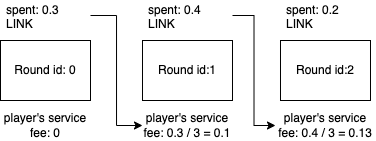
\includegraphics[scale=0.8]{images/fees2.png} 
    \caption{Calculating service fees}
    \label{fig:b1}
\end{figure}
\FloatBarrier

The deposit function also has an additional safeguard - a player cannot execute it if they chose to pay greater gas price than the VRF gas lane limit.

\newpage
High level overview of actions during a single round life-cycle:
\begin{figure}[!ht]
    \centering
    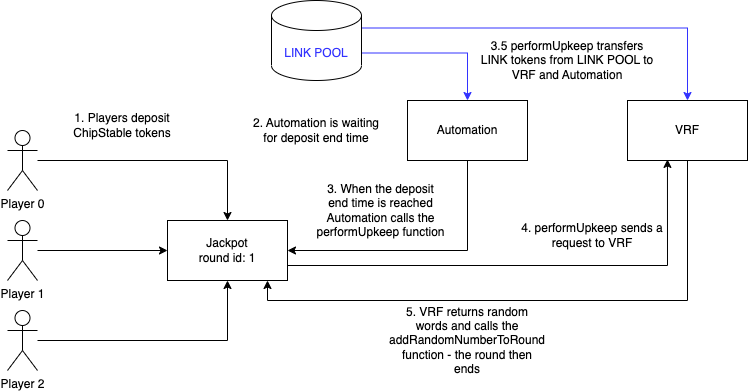
\includegraphics[scale=0.6]{images/fees.png} 
    \caption{Actions during round life-cycle}
    \label{fig:b1}
\end{figure}
\FloatBarrier


While Automation calls the performUpkeep function, the following things happen in the background:
\begin{itemize}
    \item Service fees are sent to VRF subscription and Automation Upkeep
    \item Current Automation Upkeep and current VRF subscription balances are saved to Jackpot contract, in order to calculate service fee for the next round
    \item Round closes
\end{itemize}

\textbf{NOTE}: e.g. Automation spent 0.1 LINK and VRF spent 0.2 LINK, so 0.1 LINK is sent to Automation Upkeep and 0.2 LINK is sent to VRF subscription.

\hfill

By operating on this mechanism, the Jackpot contract is fully self-sustainable - it does not need any external control to work reliably and continuously. 

\section{ChipStable}
ChipStable is the token created for the purpose of CheapChipsJackpot game. It is an ERC20\cite{erc20} token with 0 decimals.

\newpage
\printbibliography
\end{document}